%!TEX TS-program = xelatex
\documentclass[]{friggeri-cv}
\usepackage{afterpage}
\usepackage{hyperref}
\usepackage{color}
\usepackage{xcolor}
\usepackage{smartdiagram}
\usepackage{fontspec}
% if you want to add fontawesome package
% you need to compile the tex file with LuaLaTeX
% References:
%   http://texdoc.net/texmf-dist/doc/latex/fontawesome/fontawesome.pdf
%   https://www.ctan.org/tex-archive/fonts/fontawesome?lang=en
%\usepackage{fontawesome}
\usepackage{metalogo}
\usepackage{dtklogos}
\usepackage[utf8]{inputenc}
\usepackage{tikz}
% This fixes the overfull hbox
\usepackage{microtype}
\usetikzlibrary{mindmap,shadows}
\hypersetup{
    pdftitle={},
    pdfauthor={},
    pdfsubject={},
    pdfkeywords={},
    colorlinks=false,           % no link border color
    allbordercolors=white       % white border color for all
}
\smartdiagramset{
    bubble center node font = \footnotesize,
    bubble node font = \footnotesize,
    % specifies the minimum size of the bubble center node
    bubble center node size = 0.5cm,
    %  specifies the minimum size of the bubbles
    bubble node size = 0.5cm,
    % specifies which is the distance among the bubble center node and the other bubbles
    distance center/other bubbles = 0.3cm,
    % sets the distance from the text to the border of the bubble center node
    distance text center bubble = 0.5cm,
    % set center bubble color
    bubble center node color = pblue,
    % define the list of colors usable in the diagram
    set color list = {lightgray, materialcyan, orange, green, materialorange, materialteal, materialamber, materialindigo, materialgreen, materiallime},
    % sets the opacity at which the bubbles are shown
    bubble fill opacity = 0.6,
    % sets the opacity at which the bubble text is shown
    bubble text opacity = 0.5,
}

\addbibresource{bibliography.bib}
\RequirePackage{xcolor}
\definecolor{pblue}{HTML}{0395DE}

\begin{document}
\header{Mario}{Piazza}
      {Software Engineer}
      
% Fake text to add separator      
\fcolorbox{white}{gray}{\parbox{\dimexpr\textwidth-2\fboxsep-2\fboxrule}{%
.....
}}

% In the aside, each new line forces a line break
\begin{aside}
  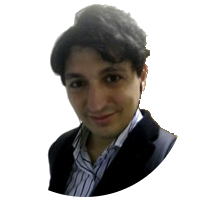
\includegraphics[scale=0.48]{img/foto_profilo.png}
  \section{Address}
    Vicolo Sortino, 24
    Sciacca, Italy
    ~
  \section{Tel}
    +39 331 2272564
    ~
  \section{Mail}
    \href{mailto:mario.piazza@mail.com}{\textbf{mario.piazza@}\\mail.com}
    ~
  \section{Links}
    %\href{http://mywebsite.com}{mywebsite.com}
    %\href{https://bitbucket.org/kyokokken}{bitbucket.org/kyokokken}
    \href{https://github.com/kyokokken}{github.com/\\\textbf {kyokokken}}
    \href{https://www.linkedin.com/in/piazzamario}{linkedin.com/in/\\\textbf {piazzamario}}
    %\href{https://gitlab.com/u/mygit}{gitlab.com/u/mygit}
    ~
  % use  \hspace{} or \vspace{} to change bubble size, if needed
  \section{Main Languages}
    \smartdiagram[bubble diagram]{
        \textbf{Java},
        \textbf{Kotlin},
        \textbf{Python},
        \textbf{Shell scripting},
        \textbf{JavaScript},
        \textbf{SQL}
        %\textbf{HTML/CSS}\\\textbf{JS/},
        %\textbf{PHP},
        %\textbf{Android},
        %\textbf{Bash}
    }
    ~
  \section{Main Tools\&\\Frameworks}
    \smartdiagram[bubble diagram]{
        \textbf{Spring},
        \textbf{Tensorflow},
        \textbf{Android},
        \textbf{JUnit},
        \textbf{Mockito},
        \textbf{Git}
    }
    ~
\end{aside}
~
\section{Profile}
{Playing with computers since I was 6. Senior Java Developer with 5+ years on real-world projects. Interested in Machine Learning applications.}

\section{Experience}
\begin{entrylist}
  \entry
    {03/19 - Now}
    {Analyst Developer}
    {Alten}
    {{\begin{itemize}
        \item {Joined a dev team using Agile methodologies at Banking clients.\\Begin development of a tool in Java 8 and Struts 2 for WebSphere 9.0 using IBM MyEclipse.}
        \item {Report building and maintenance of a legacy database written in MSSQL 2005.}
        \item {Lead developer of a Java Web Application.\\Development from scratch of a Spring Boot 2 application for translating REST-to-SOAP messages. Used TDD with Mockito, JUnit and RestAssured.}
        \item {Lead developer of a serverless Android application integrated with external services.\\ Written in Kotlin and integrated with AWS Polly and Rekognition, Scipafi and Mobbscan services.}
    \end{itemize}}
      {Skills and frameworks used:\\Java, Kotlin, Git, AWS, React Native, Struts, MyEclipse, WebSphere, Spring Boot, Tomcat, Swagger, Lombok, Hibernate, Mockito, RestAssured, JUnit, Markdown, MongoDB, Node, JavaScript, WebSphere, T-SQL, IIS, C\#, SQL Server reports (Creation of RDL)}}
  \entry
    {01/16 - 03/19}
    {IT \& Telecommunications Architect}
    {Best Continent}
    {{\\Building of network and telecommunications infrastructure.}
            {\begin{itemize}
                \item{Based on Asterisk PBX}
                \item{Configuration of 6 VoIP phones, Patton VoIP gateway and Cisco switch}
                \item{Managed regular backup and maintenance}
            \end{itemize}}
    {Helped customer integrate their systems with XML/API hotel suppliers.}
    {\\Development of a Web Application using Google App Engine for Java with authentication and caching support.}
    {\\Website development in wordpress, with creation of custom plugins and post types.}
    {\\Skills and frameworks used:\\Asterisk, CentOS, Git, Java, Spring Boot, Lombok, Thymeleaf, Hibernate, JUnit, MySQL, Wordpress, PHP}}
  \entry
    {01/08 - 01/16}
    {IT Engineer}
    {Garibaldi Relais}
    {{\\Extension of existing Excel application at accommodation business.}
    {\\Integration with external program with remote control support.}
    {\\Implementing UX improvements.}
    {\\Skills and frameworks used:\\Excel VBA, Git, Java, Spring, Android development, Hibernate, MySQL, Cordova}}
\end{entrylist}
\newpage

\section{Knowledge}
{Java, Spring, Kotlin, Android Development, Shell Scripting {\tiny(POSIX-compatible)}, Git, Maven, Gradle, AWS, Python, Hibernate, JUnit, Mockito, Struts, Node, {\tiny(No)}SQL, JavaScript, VBA for applications, C\#, Thymeleaf, React, HTML/CSS/JS, PHP, Tensorflow, Keras, \LaTeX, Markdown, AsciiDoc, Linux{\tiny(Ubuntu, Debian, CentOS)}, REST, SOAP, Vim, Jetbrains IDEs, Regex, Scrum, Functional programming, OOP, TDD, Clean code \& SOLID principles, Design Patterns}

\section{Education}
\begin{entrylist}
  \entry
    {2001 - 2008}
    {Bachelor's Degree in IT Engineering}
    {University of Palermo}
    {Score 97/110\\
    Courses included: Algorithms, Artificial Intelligence, Robotics}
%  \entry
%    {2005 - 2009}
%    {Bachelor's Degree in Computer Engineering}
%    {School}
%    {Lorem ipsum dolor sit amet, consectetur adipiscing elit, sed do eiusmod tempor incididunt ut labore et dolore magna aliqua. Ut enim ad minim veniam, quis nostrud exercitation ullamco laboris nisi ut aliquip ex ea commodo consequat\\}
%  \entry
%    {2000 - 2005}
%    {Scientific Disploma}
%    {School}
%    {Lorem ipsum dolor sit amet, consectetur adipiscing elit, sed %do eiusmod tempor incididunt ut labore et dolore magna aliqua}
\end{entrylist}

\section{Portfolio}
\begin{entrylist}
  \entry
    {2018}
    {Slide Gems}
    {Multiplatform Game (Desktop/Android/iOS/HTML)}
    {{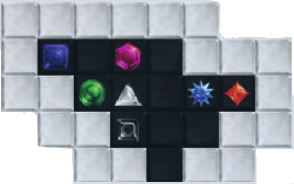
\includegraphics[scale=0.50]{img/slide_gems_snip.png}}\\\href{https://bit.ly/2Gwwct5}{\textbf{Play Store Link}}}
    
    
     
    %{Lorem ipsum.\\
    %\emph{Lorem ipsum}}
\end{entrylist}

\begin{aside}
~
~
~
%  \section{OS Preference}
%    \textbf{GNU/Linux}
\includegraphics[scale=0.40]{img/5stars.png}
%    \textbf{Unix}
\includegraphics[scale=0.40]{img/4stars.png}
%    \textbf{MacOS}
\includegraphics[scale=0.40]{img/2stars.png}
%    \textbf{Windows}
\includegraphics[scale=0.40]{img/1stars.png}
    ~
%  \section{Places Lived}
%    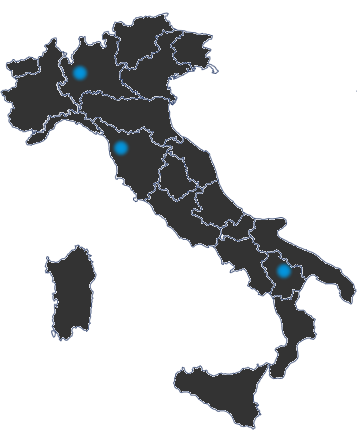
\includegraphics[scale=0.25]{img/italia.png}
    ~
  \section{Languages}
    \textbf{Italian}
\includegraphics[scale=0.40]{img/5stars.png}
    \textbf{English}
\includegraphics[scale=0.40]{img/4stars.png}
    ~
\end{aside}

%\section{Publications}
%Author, Author, Author\\
%\textbf{Lorem ipsum dolor sit amet, consectetur adipiscing elit, %sed do eiusmod tempor incididunt ut labore et dolore magna aliqua}\\
%\emph{Lorem ipsum dolor sit amet, consectetur adipiscing elit, sed do eiusmod tempor incididunt ut labore et dolore magna aliqua}
%\\
%\section{Honors \& Awards}
%\begin{entrylist}
%  \entry
%    {10/2015}
%    {Best swordsman duel}
%    {Contest}
%    {Lorem ipsum.\\
%    \emph{Lorem ipsum}}
%\end{entrylist}

\section{Certifications}
\begin{entrylist}
  \entry{}
    {05/15}
    {edX}
    {edX Honor Code Certificate for Introduction to Linux}
    %{\emph{Building a Python Search Engine}}
  \entry{}
    {08/14}
    {Coursera}
    {Algorithmic Thinking}
    %{\emph{Building a Python Search Engine}}
  \entry{}
    {08/14}
    {Coursera}
    {Principles of Computing}
    %{\emph{Building a Python Search Engine}}
  \entry{}
    {07/14}
    {Coursera}
    {Pattern-Oriented Software Architectures: Programming Mobile Services for Android Handheld Systems}
    %{\emph{Building a Python Search Engine}}
  \entry{}
    {06/14}
    {Coursera}
    {Web Application Architectures}
    %{\emph{Building a Python Search Engine}}
  \entry{}
    {03/14}
    {Coursera}
    {Programming Mobile Applications for Android Handheld Systems}
    %{\emph{Building a Python Search Engine}}
  \entry{}
    {02/14}
    {Coursera}
    {Cryptography I}
    %{\emph{Building a Python Search Engine}}
  \entry{}
    {07/13}
    {Coursera}
    {Malicious Software and its Underground Economy: Two Sides to Every Story}
    %{\emph{Building a Python Search Engine}}
  \entry{}
    {06/13}
    {Coursera}
    {Introduction to Data Science}
    %{\emph{Building a Python Search Engine}}
  \entry{}
    {12/08}
    {Cisco}
    {CCNA Exploration}
    %{\emph{Building a Python Search Engine}}
\end{entrylist}
\newpage
\section{About my programming style}
I value testing and documentation\\
I write documentation of everything I do\\
I use TDD as a design tool\\
I try to follow SOLID and clean code principles as much as possible\\
I know most of the common Design Patterns\\

\section{Other Info}
For the Italian job market:\\
\emph{Si autorizza il trattamento delle informazioni contenute nel curriculum in conformità alle disposizioni previste dal d.lgs. 196/2003. Si dichiara altresì di essere consapevole che, in caso di dichiarazioni non veritiere, si è passibili di sanzioni penali ai sensi del DPR 445/00 oltre alla revoca dei benefici eventualmente percepiti.}
\\
\begin{flushleft}
\emph{June 1st, 2019}
\end{flushleft}
\begin{flushright}
\emph{Mario Piazza}
\end{flushright}

\end{document}

